\documentclass{classes/mybeamer}

\title{
    ピタゴラス数に対するフライ曲線の\\
    Mordell-Weil群について
}
\author{八木 颯仁}
\institute{慶應義塾大学 栗原研究室 修士1年}
\date{\today}

\begin{document}

\begin{frame}
    \titlepage
\end{frame}

\begin{frame}{発表の内容と動機}
    フライ曲線とは楕円曲線の一種であり、フェルマーの最終定理の証明において重要な役割を果たした。
    フライ曲線はフェルマー方程式の解に対応して定まる「存在しない」曲線である。
    私はフライ曲線の方程式を少し変形し、ピタゴラス数に対して定まる「存在する」楕円曲線について研究し、
    そのMordell-Weil群(後で定義を与える)の構造について\textbf{独自の結果を得た}。

    \vspace{1cm}

    \begin{itemize}
        \item 楕円曲線とは
        \item フライ曲線とは
        \item Torsion subgroup
        \item ランク
        \item 具体例
    \end{itemize}
\end{frame}

\begin{frame}{楕円曲線とは}
    $\mathbb{Q}$上の\color{blue}\textbf{楕円曲線}\color{black}$E$とは次のような形の方程式で表される曲線である。
    \begin{equation}
        E: y^2 = x^3 + ax^2 + bx+c \quad (a, b, c \in \mathbb{Q}).
    \end{equation}
    ただし右辺は$\overline{\mathbb{Q}}$において重根を持たないとする。

    \vspace{1cm}

    $P, Q \in E$とし、$L$を$P$と$Q$を通る直線とするとき$L$と$E$は重複度を込めてちょうど3点で交わる。
    そこで$L$と$E$のもう1つの交点を$R$とし、$R$と$x$軸について対称な点を$P+Q$と定義する。

    $E$上の有理点全体に無限遠点$\mathcal{O}$を加えた集合を\color{blue}\textbf{Mordell-Weil群}\color{black}と呼び、$E(\mathbb{Q})$と書く。
    $E(\mathbb{Q})$は上の演算により$\mathcal{O}$を単位元としてアーベル群をなす。
\end{frame}

\begin{frame}
    \begin{figure}[htbp]
        \centering
        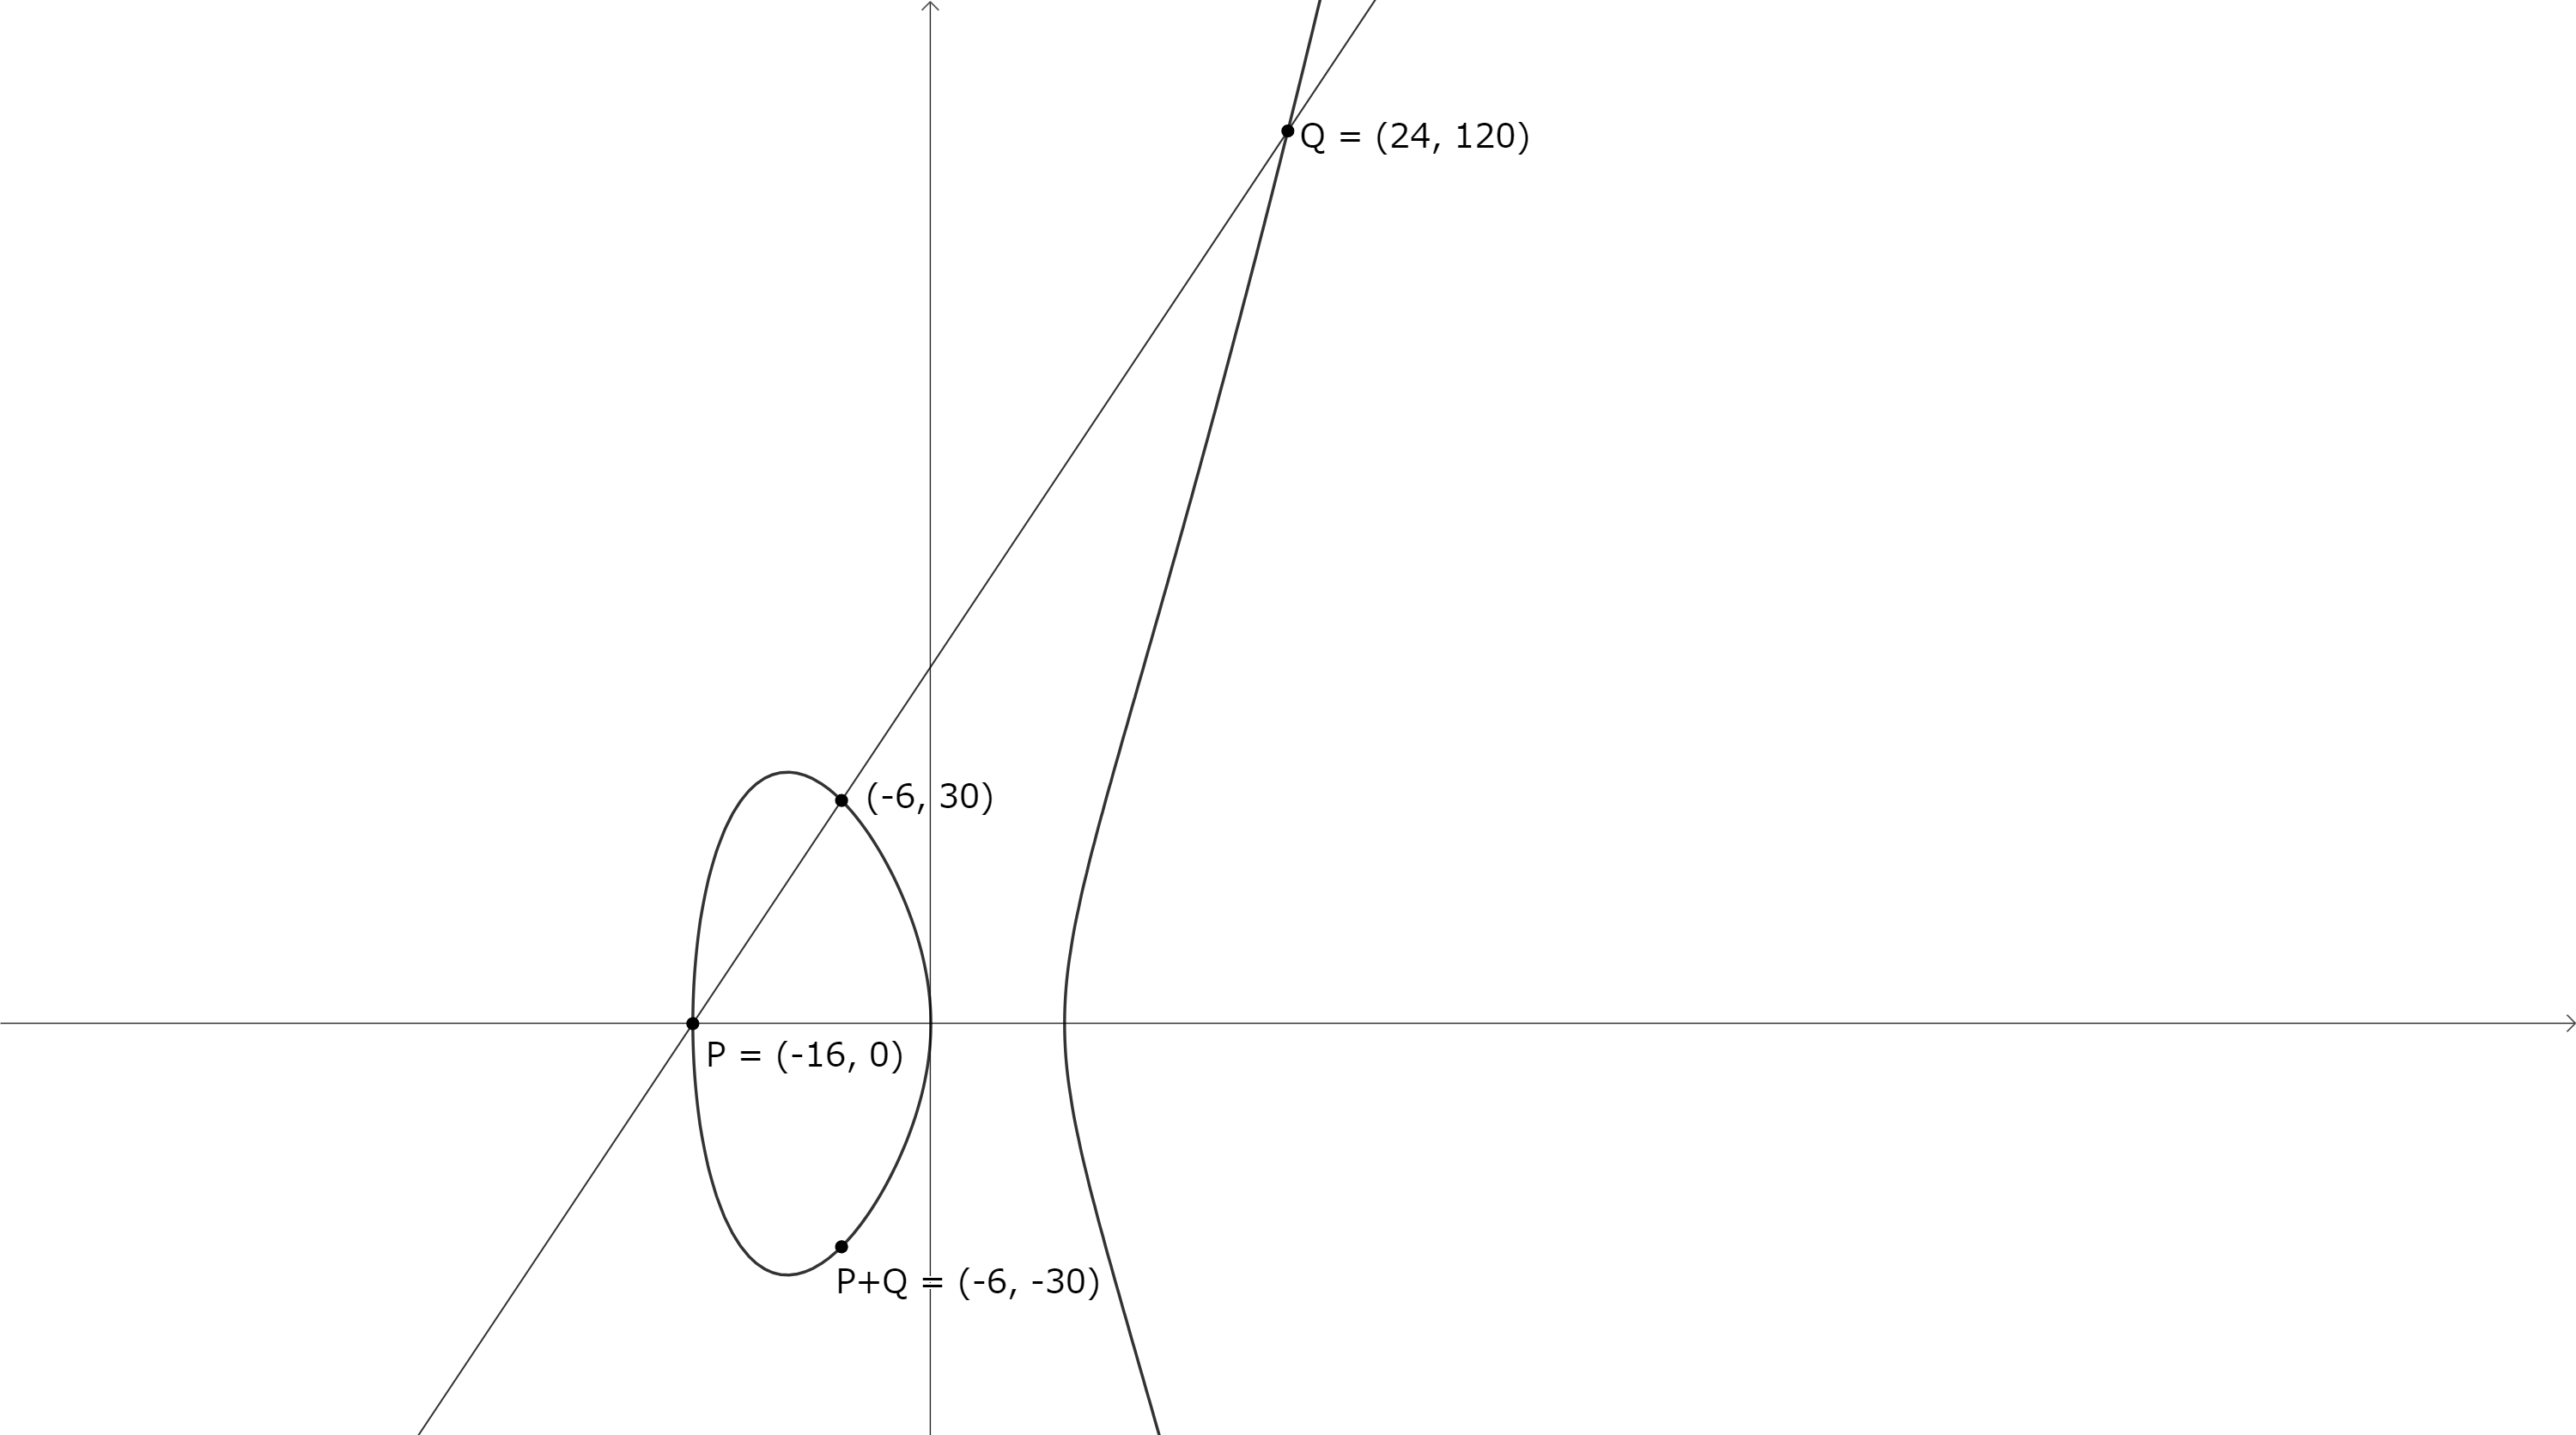
\includegraphics[keepaspectratio, height=8.5cm]{figures/3-4-5.png}
        \vspace{-1.5cm}
        \caption{
            \rightline{
                $E: y^2 = x(x-3^2)(x+4^2)$
            }
        }
    \end{figure}
\end{frame}

\begin{frame}{楕円曲線とは}
    \begin{thm}[Mordell]
        $E(\mathbb{Q})$は有限生成アーベル群であり, したがって次のように書ける。
        \begin{equation}
            E(\mathbb{Q}) \simeq \mathbb{Z}^r \times E(\mathbb{Q})_{\mathrm{tors}}.
        \end{equation}
        ただし$E(\mathbb{Q})_\mathrm{tors}$は$E(\mathbb{Q})$の元のうち位数が有限のもの全体の集合である。

        $r$を$E(\mathbb{Q})$の\color{blue}\textbf{ランク}\color{black}、$E(\mathbb{Q})_\mathrm{tors}$を\color{blue}\rm{\textbf{torsion subgroup}}\color{black}と呼ぶ。
    \end{thm}
    \begin{thm}[Mazur]
        \label{thm:mazur}
        $E(\mathbb{Q})_{\text{tors}}$は次のいずれかに同型である。
        \begin{equation}
            \begin{aligned}
                (1)\quad & \mathbb{Z}/n\mathbb{Z}                                &  & (1 \leq n \leq 10\,\mbox{もしくは}\,n=12), \\
                (2)\quad & \mathbb{Z}/2\mathbb{Z} \times \mathbb{Z}/2n\mathbb{Z} &  & (1 \leq n \leq 4).
            \end{aligned}
        \end{equation}
    \end{thm}
\end{frame}

\begin{frame}{フライ曲線とは}
    \begin{dfn*}
        フェルマー方程式
        \begin{equation}
            x^n + y^n = z^n, \quad xyz \neq 0, \quad n \geq 3
        \end{equation}
        の解$(x, y, z)=(a,b,c)$に対し、
        \begin{equation}
            y^2 = x (x-a^n) (x+b^n)
        \end{equation}
        は楕円曲線を与える。これを\color{blue}\textbf{フライ曲線}\color{black}と呼ぶ。
    \end{dfn*}
    \begin{dfn*}
        $(a,b,c)$を以下を満たす有理数の$3$つ組であるとする。
        \begin{equation}
            \label{eq:pythagorean_triple}
            a^2+b^2=c^2, \quad abc \neq 0.
        \end{equation}
        次の方程式で与えられる楕円曲線$E/\mathbb{Q}$を、\color{blue}\textbf{ピタゴラス数に対するフライ曲線}\color{black}と呼ぶことにする。
        \begin{equation}
            \label{eq:pythagorean_frey_curve}
            E: y^2 = x (x-a^2) (x+b^2) = x^3 + (b^2 - a^2) x^2 - a^2b^2x.
        \end{equation}
    \end{dfn*}
\end{frame}

\begin{frame}{フライ曲線とは}
    互いに素な正の整数$a_0,b_0,c_0$が$a_0^2+b_0^2=c_0^2$を満たすとき、$(a_0,b_0,c_0)$を原始ピタゴラス数と呼ぶ。
    \eqref{eq:pythagorean_triple}を満たす有理数の$3$つ組$(a, b, c)$に対し、
    $s\in \mathbb{Q}^\times$と原始ピタゴラス数$(a_0, b_0, c_0)$が存在し、
    \begin{equation}
        (a,b,c) = (sa_0, sb_0, sc_0)
    \end{equation}
    と書ける。 $(x,y)\mapsto (s^{-2}x, s^{-3}y)$という変換により$y^2=x(x-a^2)(x+b^2)$は
    \begin{equation}
        Y^2 = X (X-a_0^2) (X+b_0^2)
    \end{equation}
    に$\mathbb{Q}$上同型である。
    したがってこの後の証明中では\color{red}$(a,b,c)$が原始ピタゴラス数であると仮定して一般性を失わない。\color{black}
\end{frame}

\begin{frame}{Torsion subgroup}
    ピタゴラス数に対するフライ曲線について\textbf{独自に以下の結果を得た}。
    \begin{thm}\label{thm:torsion}
        $E/\mathbb{Q}$をピタゴラス数に対するフライ曲線とするとき以下が成り立つ。
        \begin{equation}
            \begin{split}
                E(\mathbb{Q})_{\mathrm{tors}} &= \{\mathcal{O}, (0,0), (a^2,0), (-b^2,0), (a^2+ac, \pm ac(a+c)), (a^2-ac, \pm ac(a-c))\}\\
                &= \langle(0,0), (a^2+ac, ac(a+c))\rangle\\
                &\simeq \mathbb{Z}/2\mathbb{Z} \times \mathbb{Z}/4\mathbb{Z}.
            \end{split}
        \end{equation}
    \end{thm}
    \begin{alertblock}{}
        \begin{itemize}
            \item 定義よりすぐに「$P=(x,y)\in E(\mathbb{Q})\text{の位数が}2\iff y=0$」は分かる。
            \item 楕円曲線の演算は幾何的に定義したが、係数を使って具体的に書けることが知られており、
                  \begin{equation}
                      x(2P) = \frac{a^4 b^4 + 2 a^2 b^2 x^2 + x^4}{4 x (x-a^2) (x+b^2)} = a^2
                  \end{equation}
                  という方程式を解くことで4-torsion pointsも具体的に求めることができた。
        \end{itemize}
    \end{alertblock}
\end{frame}

\begin{frame}{Theorem \ref{thm:torsion}の証明}
    \theoremstyle{definition}
    \newtheorem*{MazurTheorem}{Theorem \ref{thm:mazur} (Mazur, 再掲)}
    \begin{MazurTheorem}
        $E(\mathbb{Q})_{\text{tors}}$は次のいずれかに同型である。
        \begin{equation}
            \begin{aligned}
                (1)\quad & \mathbb{Z}/n\mathbb{Z}                                &  & (1 \leq n \leq 10\,\mbox{もしくは}\,n=12), \\
                (2)\quad & \mathbb{Z}/2\mathbb{Z} \times \mathbb{Z}/2n\mathbb{Z} &  & (1 \leq n \leq 4).
            \end{aligned}
        \end{equation}
    \end{MazurTheorem}
    $\mathbb{Z}/2\mathbb{Z}\times\mathbb{Z}/4\mathbb{Z} \subset E(\mathbb{Q})_\mathrm{tors}$が分かった時点で、
    $E(\mathbb{Q})_\mathrm{tors}$の可能性は
    \begin{equation}
        \mathbb{Z}/2\mathbb{Z} \times \mathbb{Z}/4\mathbb{Z} \quad\text{または}\quad \mathbb{Z}/2\mathbb{Z} \times \mathbb{Z}/8\mathbb{Z}
    \end{equation}
    のいずれかに絞られる。したがってあとは8-torsion pointsが存在しないことを示せばよい。

    \begin{alertblock}{}
        8-torsion pointsが存在すると仮定すると、以下の方程式が非自明な整数解を持つことが示せる。
        \begin{equation}
            x^4 + y^2 = z^4.
        \end{equation}
        しかしこの方程式は非自明な整数解を持たないことが知られている \cite{ref:aec}。
    \end{alertblock}
\end{frame}

\begin{frame}{ランク}
    \begin{thm}[$(a,b,c)=(3,4,5)$]\rm
        \label{eg:3-4-5}
        次の楕円曲線
        \begin{equation}
            E: y^2 = x (x-3^2) (x+4^2) = x^3 + 7 x^2 - 144 x
        \end{equation}
        のMordell-Weil群$E(\mathbb{Q})$は
        \begin{equation}
            E(\mathbb{Q}) \simeq \mathbb{Z}/2\mathbb{Z} \times \mathbb{Z}/4\mathbb{Z}
        \end{equation}
        となる。
        特にランクは$0$である。
    \end{thm}
    \begin{thm}[$(a,b,c)=(15,8,17)$]\rm
        \label{eg:15-8-17}
        次の楕円曲線
        \begin{equation}
            E: y^2 = x (x-15^2) (x+8^2) = x^3 -161 x^2 - 14400 x
        \end{equation}
        のMordell-Weil群$E(\mathbb{Q})$は
        \begin{equation}
            E(\mathbb{Q}) \simeq \mathbb{Z} \times \mathbb{Z}/2\mathbb{Z} \times \mathbb{Z}/4\mathbb{Z}
        \end{equation}
        となる。
        特にランクは$1$である。
    \end{thm}
\end{frame}

\begin{frame}{ランク}
    \begin{dfn*}{}
        \begin{itemize}\rm
            \item 一般的にランクを求めるのは難しい(アルゴリズムは知られていない)。
            \item いつでも使えるわけではないがSilvermanの教科書 \cite{ref:naskreckiphd}で紹介されている手法を紹介する。
        \end{itemize}
    \end{dfn*}

    $\mathbb{Q}$上の楕円曲線$E: y^2=x^3+Ax^2+Bx$に対し、
    \begin{equation}
        \begin{split}
            &S \coloneq \{\infty, 2\} \cup \{p: \text{素数} \mid v_p(\Delta) \geq 1 \}, \\
            &\mathbb{Q}(S,2) \coloneq \left\{ b\in\mathbb{Q}/\mathbb{Q}^{\times 2} \mid \forall p \notin S, v_p(b)\equiv 0 \pmod 2 \right\}
        \end{split}
    \end{equation}
    とおき、
    \begin{equation}
        \phi: E \to E', \quad \hat{\phi}: E' \to E, \quad \hat{\phi}\circ\phi=[2]\quad\text{(2倍写像)}
    \end{equation}
    なる楕円曲線$E'/\mathbb{Q}$と$\phi: \text{2-isogeny}$(具体的な与え方は省略)を考えて
    \begin{equation}
        \begin{split}
            &C_d: dw^2 = d^2 - 2Adz^2 + (A^2-4B)z^4: \quad \text{Homogeneous space} \\
            &\color{red}S^{(\phi)}(E/\mathbb{Q}) \coloneq \left\{ d\in \mathbb{Q}(S,2) \mid \forall v \in S, C_d(\mathbb{Q}_v)\neq\varnothing \right\}: \quad \text{Selmer群}\color{black}
        \end{split}
    \end{equation}
    と定義する。
    \begin{alertblock}{}
        \begin{equation}
            \# S < \infty, \quad \# \mathbb{Q}(S,2) < \infty
        \end{equation}
    \end{alertblock}
\end{frame}

\begin{frame}{ランク}
    次の完全系列が存在する。
    \begin{eg*}
        \begin{equation}
            \label{eq:selmer-sequence}
            0 \to E'(\mathbb{Q})/\phi(E(\mathbb{Q})) \xrightarrow{\delta} S^{(\phi)}(E/\mathbb{Q}) \to \Sha(E/\mathbb{Q})[\phi] \to 0
        \end{equation}
    \end{eg*}
    $S^{(\phi)}(E/\mathbb{Q})$が求まり、運良く$\delta$が全射であれば$E'(\mathbb{Q})/\phi(E(\mathbb{Q}))$が求まる。

    $E'(\mathbb{Q})/\phi(E(\mathbb{Q}))$と、$E$と$E'$を入れ替えて同様の計算をすることで$E(\mathbb{Q})/\hat{\phi}(E'(\mathbb{Q}))$が求まったとする。
    このとき以下の完全系列
    \begin{eg*}
        \begin{equation}
            \label{eq:two-isogeny-sequence}
            \frac{E'(\mathbb{Q})}{\phi(E(\mathbb{Q}))} \xrightarrow{\hat{\phi}} \frac{E(\mathbb{Q})}{2E(\mathbb{Q})} \to \frac{E(\mathbb{Q})}{\hat{\phi}(E'(\mathbb{Q}))} \to 0.
        \end{equation}
    \end{eg*}
    より運が良ければ$E(\mathbb{Q})/2E(\mathbb{Q})$が求まる。したがって$E(\mathbb{Q})$の生成元の数が分かる。
    ピタゴラス数に対するフライ曲線のtorsion subgroupの生成元の数は2であると分かっていたのでランクも求まる。
\end{frame}

\begin{frame}{Theorem \ref{eg:3-4-5}の証明}
    \begin{eg*}
        \begin{equation}
            S = \{\infty, 2, 3, 5\}, \quad
            \mathbb{Q}(S, 2) = \{\pm 1, \pm 2, \pm 3, \pm 5, \pm 6, \pm 10, \pm 15, \pm 30\},
        \end{equation}
        \begin{align}
            S^{(\phi)}(E/\mathbb{Q}) \coloneq \left\{ d\in \mathbb{Q}(S,2) \mid \forall v \in S, C_d(\mathbb{Q}_v)\neq\varnothing \right\}.
        \end{align}
    \end{eg*}
    たとえば$d=5$に対して、
    \begin{equation}
        C_5: w^2 = 5 - 14z^2 + 125z^4
    \end{equation}
    は$\mathbb{Q}_3$上で解を持たない(分母を払った上で$\bmod\,3$で解を持たないというのと同じような意味である)ので$5\notin S^{(\phi)}(E/\mathbb{Q})$である。
    実際$z$の$3$進付値が負(分母が$3$で割り切れる)とすると、分母を払って
    \begin{equation}
        1 \equiv w'^2 \equiv 125z'^4 \equiv 2 \pmod 3
    \end{equation}
    となり矛盾。一方$z\in \mathbb{Z}$のとき
    \begin{equation}
        \begin{aligned}
            z & \equiv 0 \pmod 3     & \Rightarrow & \quad w^2 \equiv 5 \equiv 2 \pmod 3,          \\
            z & \equiv \pm 1 \pmod 3 & \Rightarrow & \quad w^2 \equiv 5 -14 +125 \equiv  2 \pmod 3 \\
        \end{aligned}
    \end{equation}
    でありやはり矛盾。

    これをすべての$d\in \mathbb{Q}(S,2)$について計算し、さらに$E$と$E'$を入れ替えて同様の計算をする。
\end{frame}

\begin{frame}{Theorem \ref{eg:15-8-17}の証明}
    $(a,b,c)=(15,8,17)$のときは
    \begin{eg*}
        \begin{equation}
            \begin{split}
                S &= \{\infty, 2, 3, 5, 17\}, \\
                \mathbb{Q}(S,2) &= \left\{\pm1, \pm2, \pm3, \pm 5, \pm6, \pm10, \pm15, \pm17, \pm30, \pm34, \pm 51, \pm 85, \pm 102, \pm 170, \pm255, \pm510 \right\},
            \end{split}
        \end{equation}
        \begin{align}
            S^{(\phi)}(E/\mathbb{Q}) \coloneq \left\{ d\in \mathbb{Q}(S,2) \mid \forall v \in S, C_d(\mathbb{Q}_v)\neq\varnothing \right\}.
        \end{align}
    \end{eg*}
    とさらに$d$の候補が増えて、非常に多くの計算が必要になる。
\end{frame}

\begin{frame}{今後の展望}
    \begin{itemize}
        \item ピタゴラス数に対するフライ曲線でランクが$0$のものは無限個存在するか?
        \item ピタゴラス数に対するフライ曲線でランクが$1$のものは無限個存在するか?
        \item ピタゴラス数に対するフライ曲線でランクが$2$以上のものは存在するか?
    \end{itemize}
    \begin{alertblock}{}
        30個程の原始ピタゴラス数に対しデータベース \cite{lmfdb}で確認した中では、ランクは$0$と$1$のものしか出てこなかった。
    \end{alertblock}
    \begin{itemize}
        \item ランクが$0$になる$(a,b,c)$の十分条件を与えることはできるか?
        \item 他のピタゴラス数に付随する楕円曲線の族についてはどうか?
    \end{itemize}
    \begin{alertblock}{}
        たとえば
        \begin{equation}
            E: y^2 = x (x - a^2) (x - b^2)
        \end{equation}
        のランクは常に$1$以上であることが知られている \cite{ref:kodaira1963-3}。
        $a,b$に条件を付けることにより、ランクが$2$以上のものも無限個存在することが分かっている \cite{ref:yoshida}。
    \end{alertblock}
\end{frame}

\begin{frame}{参考文献}
    \scriptsize
    \beamertemplatetextbibitems
    \bibliographystyle{junsrt}
    \bibliography{references}
\end{frame}
\end{document}
